\subsection{Recorded-best trajectory and cumulative acceptance rate}\label{app:acceptance-over-rounds}

\begin{figure*}[t]
  \centering
  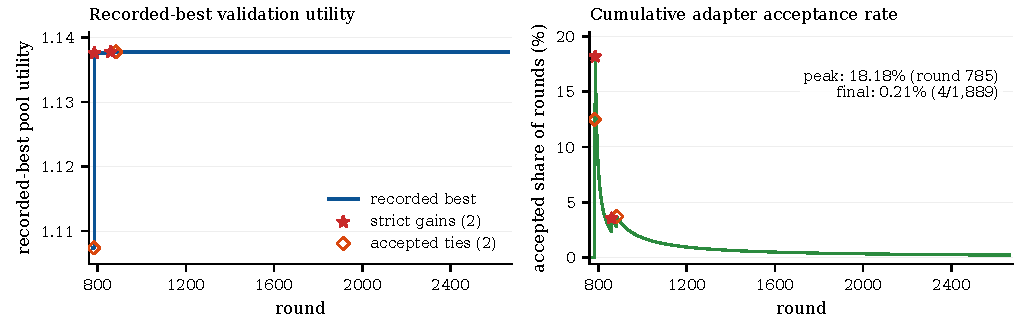
\includegraphics[width=\textwidth]{figures/fig_fw_acceptance_over_rounds.pdf}
  \caption{\textbf{Recorded-best validation utility and cumulative adapter acceptance rate over rounds.}
  Both panels use the same \num{1889} consecutive admission rounds, 775--2663, as
  \cref{fig:fw-validation}, adding no observations. Left: post-decision
  recorded-best validation pool utility, with stars at strict gains (rounds
  785 and 859) and hollow diamonds at accepted ties (rounds 782 and 882).
  Right: cumulative accepted share of elapsed rounds (\%), which peaks at
  18.18\% at round 785 and falls to 0.21\% ($4/\num{1889}$) across the
  subsequent \num{1781} rejected rounds. These are development admission
  aggregates, not independent first-proposal comparisons.}
  \label{fig:fw-acceptance-over-rounds}
\end{figure*}
\begin{figure*}[t]
  \centering
  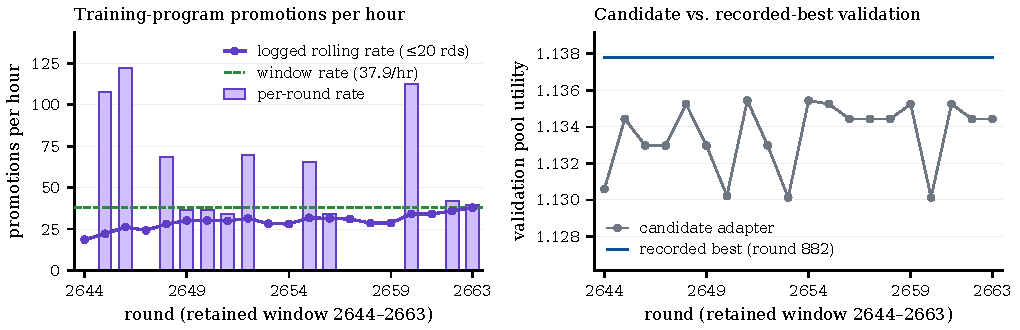
\includegraphics[width=\textwidth]{figures/fig_fw_promotions_per_hour.pdf}
  \caption{\textbf{Training-program promotions per hour and adapter validation trajectory.}
  Left: logged rolling and per-round strict training-program promotions per hour.
  Right: candidate and recorded-best adapter validation pool utility. Both panels
  cover the 20 consecutive completed rounds 2644--2663 (21 strict promotions
  over \num{1994.54}\,s of logged wall time, or 37.90 promotions per hour, with
  zero adapter admissions).}
  \label{fig:fw-promotions-per-hour}
\end{figure*}

\Cref{fig:fw-acceptance-over-rounds} provides a companion view of the
\num{1889} consecutive admission rounds, 775--2663, plotted in
\cref{fig:fw-validation}. It adds no new observations. The left panel
isolates the post-decision recorded-best validation pool utility step
curve across the two strict improvements (rounds 785 and 859, reaching
1.1376 and 1.1378 from the initial 1.1074) and the two accepted ties
(rounds 782 and 882). The right panel tracks the cumulative share of
elapsed rounds accepted up to each round: the cumulative rate reaches
18.18\% at round 785 ($2/11$ rounds), stands at 3.70\% at the last
accepted tie ($4/108$ at round 882), and declines across the \num{1781}
subsequent rejected rounds to 0.21\% ($4/\num{1889}$) by round 2663.
Binding the admission log to a qualified runtime and testing independent
first-proposal transfer remain pending (\cref{sec:method-status}).
